\section{Control Function (CF) Estimation of CM Effects}
\label{sec:controlfun}
A conventional approach to estimating CM effects involves a two-stage approach to estimating the ADE and the AIE: the first-stage $Z \to D$ and the second-stage $Z, D \to Y$.
A CF approach is a simple and intuitive addition to this approach: including the CF terms $\lambda_0, \lambda_1$ in the second-stage regression to address selection-into-mediator.

This section presents two practical estimation strategies.
First, I demonstrate how to estimate CM effects with an assumed distribution of error terms, focusing on the Heckman selection model as the leading case.
Second, I consider a more flexible semi-parametric approach that avoids distributional assumptions --- at the cost of semi-parametrically estimating the corresponding CFs.
While both methods effectively address the selection bias issues detailed in previous sections, they differ in their implementation complexity, efficiency, and underlying assumptions.

\subsection{Parametric CF}
A parametric CF solves the identification problem by assuming a distribution for the unobserved error terms in the first-stage selection model, and modelling selection based on this distribution.
The Heckman selection model is the most pertinent example, assuming the normal distribution for unobserved errors \cite{heckman1979sample}.
A parametric CF using other distributions works in exactly the same manner, replacing the relevant density functions for an alternative distribution as needed.
As such, this section focuses exclusively on the Heckman selection model.

The Heckman selection model assumes unobserved errors $V_i$ follow a normal distribution, so estimates the first-stage using a probit model.
\[ \Probgiven{D_i = 1}{Z_i, \vec X_i}
    = \Phi \big( \phi + \bar\pi Z_i + \vec\zeta' \vec X_i \big), \]
where $\Phi(.)$ is the cumulative density function for the normal distribution, and $\phi, \bar\pi, \vec\zeta$ are parameters estimated with maximum likelihood.

From this probit first-stage, we construct an estimate of the inverse Mills ratio terms to serve as the CFs.
These terms capture the correlation between unobserved factors influencing both mediator selection and outcomes, when the errors are normally distributed.
\[ \hat \lambda_0 = 1 - \Phi^{-1} \left( \hat\phi + \hat{\bar\pi} Z_i + \hat{\vec\zeta}' \vec X_i \right), \;\;\;\;
\hat \lambda_1 = \Phi^{-1} \left( \hat\phi + \hat{\bar\pi} Z_i + \hat{\vec\zeta}' \vec X_i \right). \]
Lastly, the second-stage is estimated with OLS, including the estimated CFs,
\[ Y_i = \alpha + \beta D_i + \gamma Z_i + \delta Z_i D_i + \vec\varphi' \vec X_i^- 
    + \rho_0(1-D_i) \hat \lambda_0 + \rho_1 D_i \hat \lambda_1 + \varepsilon_i. \]
The resulting ADE and AIE estimates are composed from sample estimates of the terms in Theorem \ref{thm:cf-identification},
\[ \hat{\text{ADE}}
    = \hat{\gamma} + \hat{\delta}\,\bar D_i, \;\;\;\;
    \hat{\text{ADE}}
    = \hat{\bar\pi}\; \Big(
        \hat{\beta} + \hat{\delta}\,\bar Z_i 
        + \hat \Gamma \big( \hat\pi(0;\vec X_i), \hat\pi(1;\vec X_i) \Big) \]
where $\bar D_i = \frac1N \sum_{i=1}^N D_i$, $\bar Z_i = \frac1N \sum_{i=1}^N Z_i$, and $\hat\pi \big(z';\vec X_i \big) = \Phi \big( \hat\phi + \hat{\bar\pi} z' + \hat{\vec\zeta}' \vec X_i \big)$ are the predictions for the probit first-stage, and $\hat\Gamma(.,.)$ is the estimate of the complier adjustment term using the estimated CF $\hat\lambda_1$.

The standard errors for estimates can be computed using the delta method \citep{heckman1979sample}.
Specifically, we account for both the sampling variability in the coefficient estimates and the fact that the CFs themselves are estimated in the first-stage.
This approach yields $\sqrt{n}$-consistent estimates when the underlying error terms follow a bivariate normal distribution --- i.e., when $\lambda_0, \lambda_1$ and $\hat\pi$ are correctly modelled by the probit first-stage.
Errors can also be estimated by the bootstrap, including estimation of both the first and second-stage within each bootstrap iteration.

In practice, a parametric CF approach is simple to implement using standard statistical packages.
The key advantage is computational simplicity and efficiency, particularly in moderate-sized samples.
However, this comes at the cost of strong distributional assumptions.
For example, if the error terms deviate substantially from joint normality, the estimates may be biased.

\subsection{Semi-parametric CF}
Note Nancy Heckamn (1986) gives $\sqrt{n}$-consistency of splines.
For settings where researchers are concerned about distributional assumptions, a semi-parametric control function approach offers greater flexibility.
This method maintains the same identification strategy but avoids assuming a specific parametric error distribution.

It's worth noting that this approach is essentially an MTE approach (Marginal Treatment Effect, developed by Heckman and Vytlacil, 1999, 2005) applied to a causal mediation setting. Just as the semi-parametric local IV approach uses variation in instruments to identify marginal treatment effects across different resistance-to-treatment margins, our semi-parametric CF approach identifies mediation effects across the distribution of unobserved mediator gains. This connection to the MTE literature provides a conceptual bridge between the instrumental variables literature and causal mediation analysis.

The first stage estimates the mediator equation using flexible methods:
\[ \Egiven{D_i}{Z_i, \vec X_i^-, \vec X_i^{\text{IV}}}
    = \pi\left(Z_i, \vec X_i^-, \vec X_i^{\text{IV}} \right) \]

Where $g(\cdot)$ is a flexible function that can be estimated using series approximation, kernel methods, or machine learning approaches. Here, $X_i^{IV}$ represents instrumental variables that affect mediator costs but not benefits, and $X_i^{-}$ represents other control variables. 

\subsection{Validation of the CF assumptions via 2SLS}

If the structural assumptions hold, then a 2SLS for $D \to Y$, using $\vec X^{\text{IV}}$ should give the same as a CF estimate.
If not, then a violation of the structural assumptions somewhere.
Could be put into an informal hypothesis test, where the null $\beta^\text{IV} = \beta^\text{CF}$ could be rejected.

\subsection{Percent of ATE Mediated Through $D$}
It is common to focus on AIE / ATE, which is necessarily a noisy estimate.
Indeed, the Kwon Roth gives a test to validate (though not confirm) that everything goes through AIE.
If reject, then move forward with this.

An inverse variance weighted version of AIE / ATE, which efficiently uses (1) AIE estimate (2) a function of the ADE estimate.
This addresses some of the inefficiency in estimating this term.

If you have large uncertainty in your treatment effect, then expect large uncertainty in the mechanisms behind it.
There is no avoiding the fact that a noisy ATE estimate (especially if close to zero) will mean noisy estimates of AIE / ATE.  

\subsection{Simulation Evidence}
The following simulation gives an example to show how this method works in practice.
Suppose data observed to the researcher $Z_i, D_i, Y_i, \vec X_i$ are drawn from the following data generating processes, for $i = 1, \hdots, N$, with 
$N = 500$ for this simulation.
\begin{align*}
    Z_i \sim \text{Binom}\left(0.5 \right),
    \;\; \vec X_i^- \sim N(4, 1),
    \;\; \vec X_i^{\text{IV}} \sim \text{Binom}\left( 0.5 \right), \\
    \left( U_{0,i}, U_{1,i} \right) \sim
    \text{BivariateNormal}\left( 0, 0, \sigma_0, \sigma_1, \rho \right),
    \;\; U_{C,i} \sim N(0, 0.5).
\end{align*}

Each $i$ chooses to take mediator $D_i$ by a Roy model, with following mean definitions for each $z', d' = 0, 1$.
\begin{align*}
    D_i(z') = \indicator{Y_i(z', 1) - Y_i(z', 0) \geq C_i},  \\
    \mu_{d'}\left(z' ; \vec X_i \right) = \vec X_i^- + \left( z' + d' + z' d' \right),
    \;\; \mu_{C}\left(z' ; \vec X_i \right) = 3z' + \vec X_i^- - \vec X_i^{\text{IV}}.
\end{align*}
Following \autoref{sec:applied}, these data have the following first and second-stage equations:
\begin{align*}
    D_i &= \indicator{-3Z_i - \vec X_i^{\text{IV}} + \vec X_i^-
        \geq U_{C,i} - \big( U_{1,i} - U_{0,i} \big)},  \\
    Y_i &= Z_i + D_i + Z_i D_i + \vec X_i^-
        + \left( 1 - D_i \right) U_{0,i} + D_i U_{1,i}.
\end{align*}
$Z_i$ has an effect on outcome $Y_i$, and it operates partially through mediator $D_i$.
Outcome mean $\mu_{D_i}(Z_i;.)$ contains an interaction term, $Z_i D_i$, so while both $Z_i$ and $D_i$ have constant partial effects, the ATE depends on how many $i$ choose to take the mediator.
In this simulation $\Prob{D_i = 1} = 0.437$, and $65.29\%$ of the sample are mediator compliers (where $D_i(1)=1$ and $D_i(0) = 0$).
This gives an ATE ($Z\to Y$) value of 2.58, ADE 1.44, and AIE 1.13, respectively.\footnote{
    Note that ATE $=$ ADE $+$ AIE in this setting.
    $\Prob{Z_i=1} = 0.5$ ensures this equality, but it is not guaranteed in general.
}

After $Z_i$ is assigned, $i$ chooses to take mediator $D_i$ by considering the costs and benefits --- which vary based on $Z_i$, demographic controls $\vec X_i$, and the (non-degenerate) unobserved error terms $U_{i,0}, U_{1,i}$.
As a result, sequential ignorability does not hold; the mediator is not conditionally ignorable.
Thus, a standard OLS (selection-on-observables) approach to CM does not give an estimate for how much of the $Z \to Y$ ATE goes through mediator $D$.
Instead, the OLS approach gives biased inference.
The bias in OLS estimates comes from the unobserved error terms being related.

\begin{figure}[h!]
    \caption{Simulated Distribution of CM Effect Estimates, Semi-parametric versus OLS, Relative to True Value.}
    \begin{subfigure}[c]{0.475\textwidth}
        \centering
        \caption{$\hat{\text{ADE}} - \text{ADE}$.}
        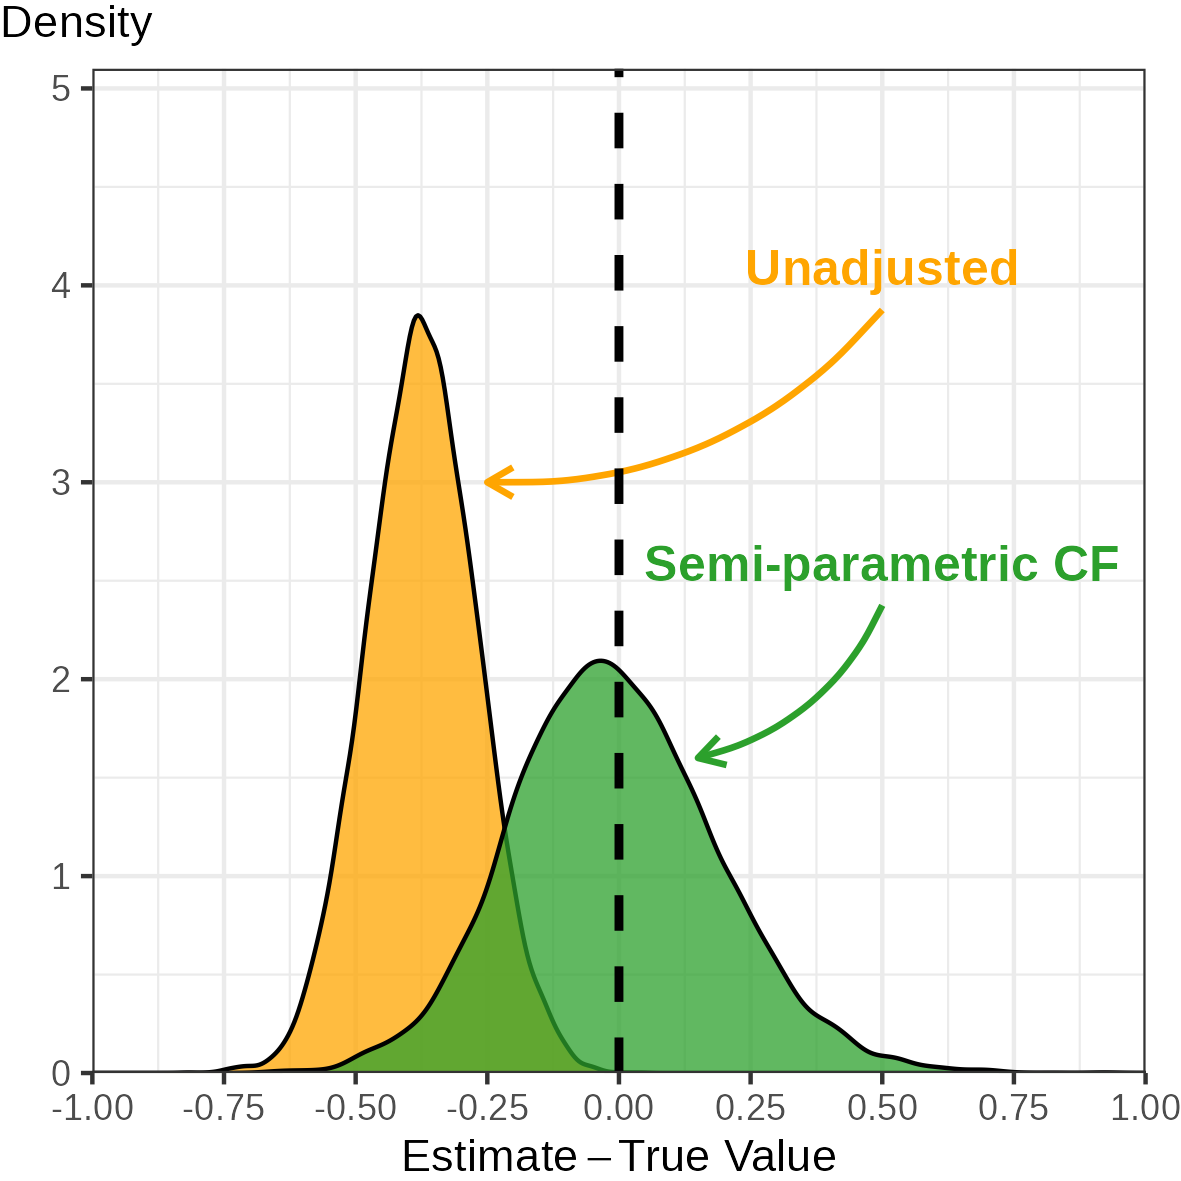
\includegraphics[width=\textwidth]{
            ../programs/simulations/sim-output/semiparametric-direct-dist.png}
    \end{subfigure}
    \begin{subfigure}[c]{0.475\textwidth}
        \centering
        \caption{$\hat{\text{AIE}} - \text{AIE}$.}
        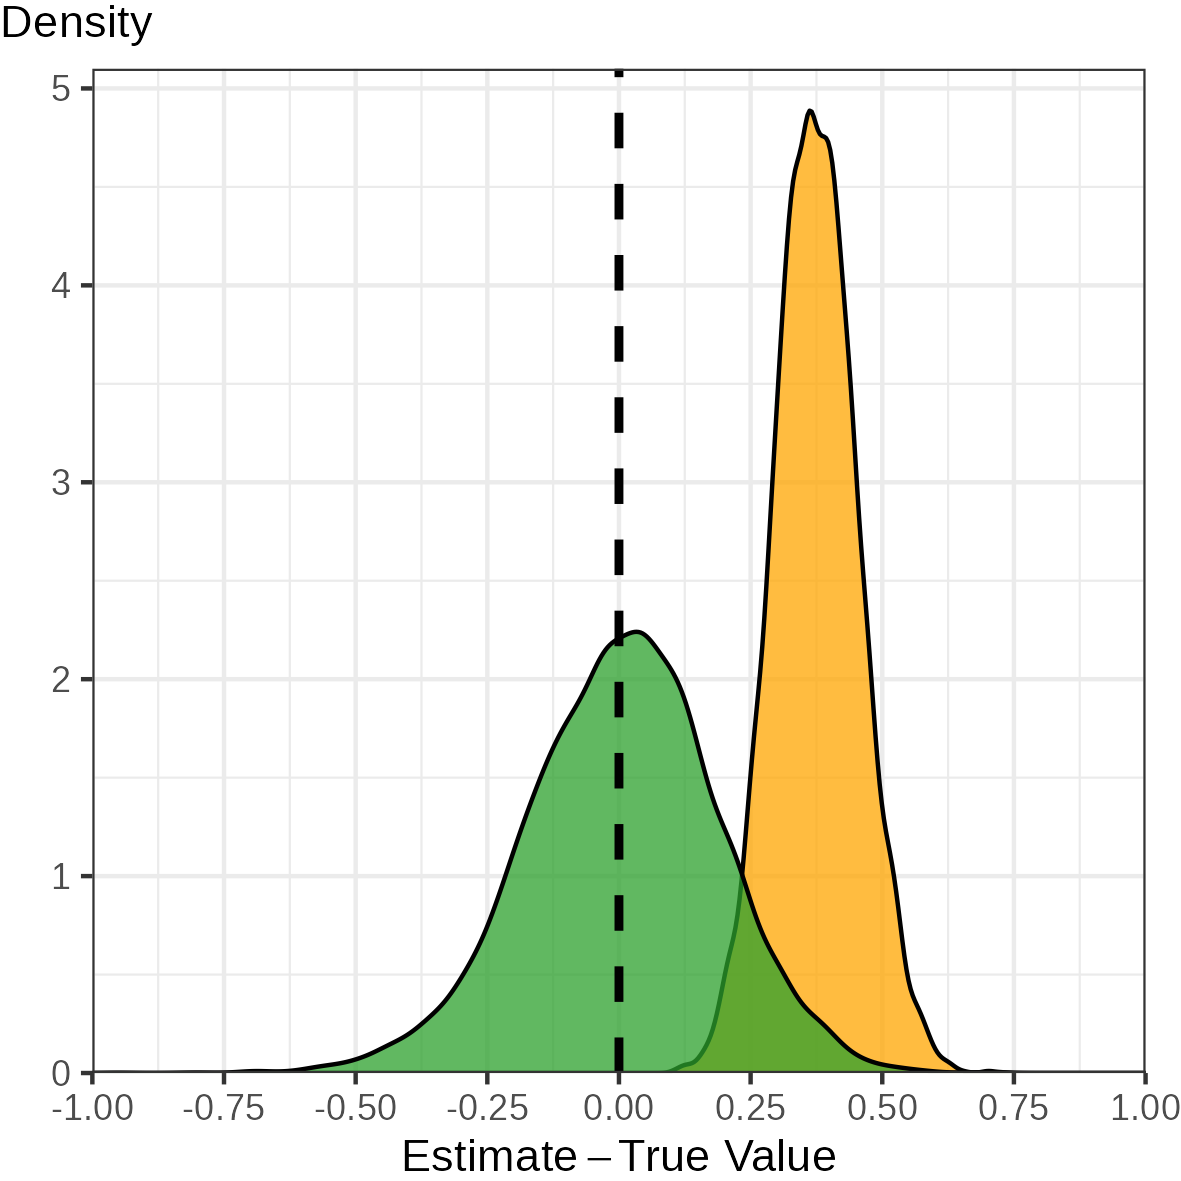
\includegraphics[width=\textwidth]{
            ../programs/simulations/sim-output/semiparametric-indirect-dist.png}
    \end{subfigure}
    \label{fig:cm-semiparametric-dist}
    \justify
    \footnotesize    
    \textbf{Note:}
    These figures show the empirical density of point estimates minus the true average effect, for 10,000 different datasets generated from a Roy model with correlated normally distributed error terms (further described in \autoref{sec:controlfun}).
    The black dashed line is the true value;
    orange is the distribution of conventional CM estimates from two-stage OLS \citep{imai2010identification},
    and green estimates with a two-stage semi-parametric CF.
\end{figure}

The CF estimator here uses the inverse Mills ratio as the CFs (i.e., a Heckman selection model); the constrained semi-parametric approach explcitily models $\lambda_1$ , and thus $\lambda_0$, with data to avoid distributional assumptions.
\autoref{fig:cm-semiparametric-dist} shows the distribution of simulated point estimates in this simulation, showing OLS against the CF approach.
The OLS approach implicitly assumes that the mediator is ignorable (when it is not), so its point estimates under and over-estimate the true ADE and AIE, respectively.
The distance between the OLS estimates and the true values are the underlying bias terms derived in \autoref{thm:selection-bias}.
In this data generating process, the OLS confidence interval do not overlap the true values for any standard level of significance.
The CF approach exhibits bias, though the 95\% confidence intervals cover the truth.

\begin{figure}[h!]
    \caption{Point Estimates of CM Effects, OLS versus CF, varying $\rho$ values with $\sigma_0 = 1, \sigma_1 = 2$ fixed.}
    \begin{subfigure}[c]{0.475\textwidth}
        \centering
        \caption{ADE.}
        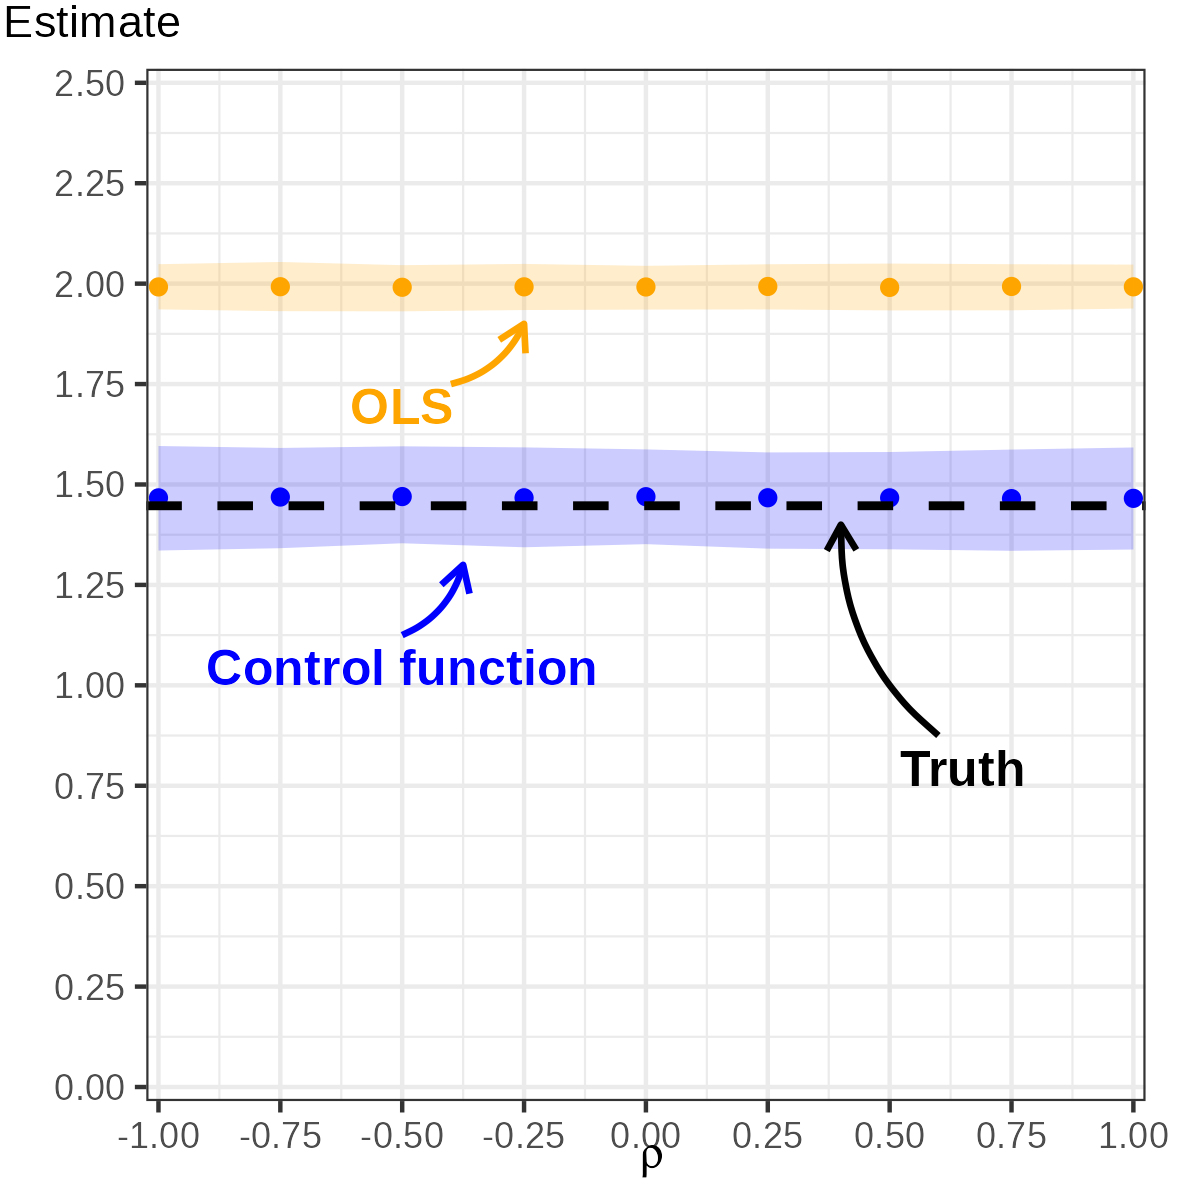
\includegraphics[width=\textwidth]{
            ../programs/simulations/sim-output/rho-directeffect-bias.png}
    \end{subfigure}
    \begin{subfigure}[c]{0.475\textwidth}
        \centering
        \caption{AIE.}
        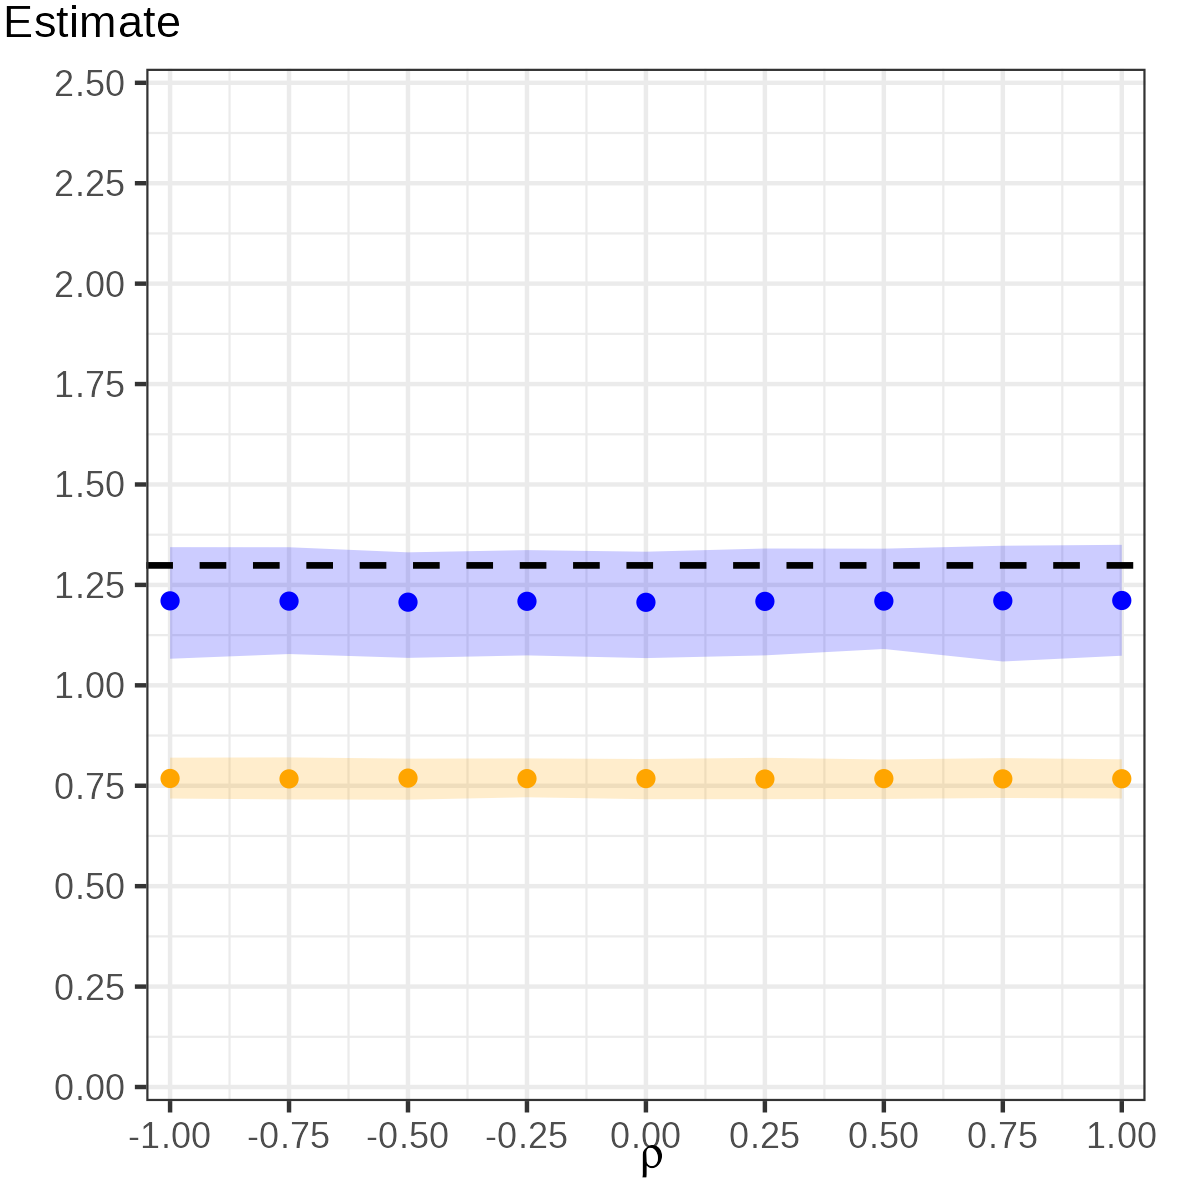
\includegraphics[width=\textwidth]{
            ../programs/simulations/sim-output/rho-indirecteffect-bias.png}
    \end{subfigure}
    \label{fig:rho-bias}
    \justify
    \footnotesize    
    \textbf{Note:}
    These figures show the OLS and CF point estimates of the ADE and AIE, for $N = 10,000$ sample size.
    The black dashed line is the true value, points are points estimates from data simulated with a given $\rho$ value and $\sigma_0 = 1, \sigma_1 = 2$, and shaded regions are the 95\% confidence intervals from 1,000 bootstraps each.
    Orange represents OLS estimates, blue the CF approach.
    The true AIE values vary with $\rho$, because $D_i(Z_i)$ compliers have higher average values of $U_{1,i} - U_{0,i}$ with greater $\rho$ values.
\end{figure}

The error terms determine the bias in OLS estimates of the ADE and AIE, so the bias varies for different values of the error-term parameters $\rho \in [-1, 1]$ and $\sigma_0, \sigma_1 \geq 0$.
\autoref{fig:rho-bias} shows CF estimates against estimates calculated by standard OLS, showing 95\% confidence intervals calculated from 1,000 bootstraps.
The point estimates of the CF do not exactly equal the true values, as they are estimates from one simulation (not averages across many simulations, as in \autoref{fig:cm-semiparametric-dist}).
The CF approach improves on OLS estimates by correcting for bias, with confidence regions overlapping the true values.\footnote{
    In the appendix, \autoref{fig:sigma-bias} shows the same simulation while varying $\sigma_1$, with fixed $\sigma_0 = 1, \rho = 0.5$.
    The conclusion is the same as for varying the correlation coefficient, $\rho$, in \autoref{fig:rho-bias}.
}
This correction did not come for free: the standard errors are significantly greater in a CF approach than OLS.
Standard errors on the AIE are larger than those for the ADE, because the AIE estimates are first-stage times second-stage estimates, so standard errors account for uncertainty in both estimates multiplied.
%(i.e., the same reasons instrumental variables estimates are less efficient than ideal OLS estimates). 
In this manner, this simulation shows the pros and cons of using the CF approach to estimating CM effects in practice.
